\documentclass[a4paper,11pt,exos]{nsi} % COMPILE WITH DRAFT
\usepackage{pifont}
\usepackage{fontawesome5}
\usepackage{hyperref}



\begin{document}
\classe{\premiere spé}
\titre{La grenouille}
\maketitle

Une grenouille fait des bonds successifs en ligne droite, en se fatiguant au fur et à mesure :
	\begin{center}
		\begin{tikzpicture}[xscale=2.8,yscale=2]
			\draw (0,0) arc (0:180:1) (1,0) arc (0:180:0.5) (1.5,0) arc (0:180:.25) (1.75,0) arc (0:180:.125) (1.875,0) arc (0:180:1/16) (2,0.05) ;
			\shade [top color = gray, bottom color=white] (-2.1,0) rectangle (2.4,-0.3);
			\draw[<->] (-2,-.20) -- node[midway,below]{\tiny 1m}(0,-.2);
			\draw[<->]  (0,-.2) -- node[midway,below]{\tiny 0.5m}(1,-.2);
			\draw[<->]  (1,-.2) -- node[midway,below]{\tiny 0.25m}(1.5,-.2);
			\draw (1.7,-.24) node{$\cdots$};
			\draw (2.1,0.05) node{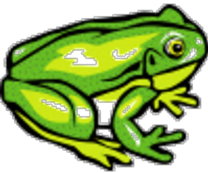
\includegraphics[width=3.5em]{frog.pdf}};
		\end{tikzpicture}
	\end{center}
	
	Le premier bond est d'un mètre. Le deuxième, $b_1$, est de $0,5$ mètres, le troisième de $0,25$ m, et ainsi de suite.\\
	On suppose que la grenouille peut faire autant de bonds que l'on désire, on se pose les questions suivantes :
	
\begin{enumerate}[label=\textbullet]
		\item 	La grenouille peut-elle aller aussi loin qu'on le désire (pourvu qu'on lui fasse faire assez de sauts) ?
		\item 	Sinon, quelle est la distance limite de la grenouille ?
\end{enumerate}

\vspace*{1cm}
\classe{\premiere spé}
\titre{Ensemble de Cantor}
\maketitle

On considère l'intervalle $\left[0\ ;1\right]$. On lui applique l'algorithme suivant :\\
	
\dleft{9.5cm}
{
	\begin{enumerate}[label=\textbullet]
		\item 	Couper l'intervalle en trois parties égales.
		\item 	Retirer la partie du milieu
		\item	Recommencer les étapes 1 et 2 avec les deux segments restants.
		\item	Recommencer les étapes 1 et 2 avec les quatre segments restants.
		\item   Etc.
	\end{enumerate}
	
}
{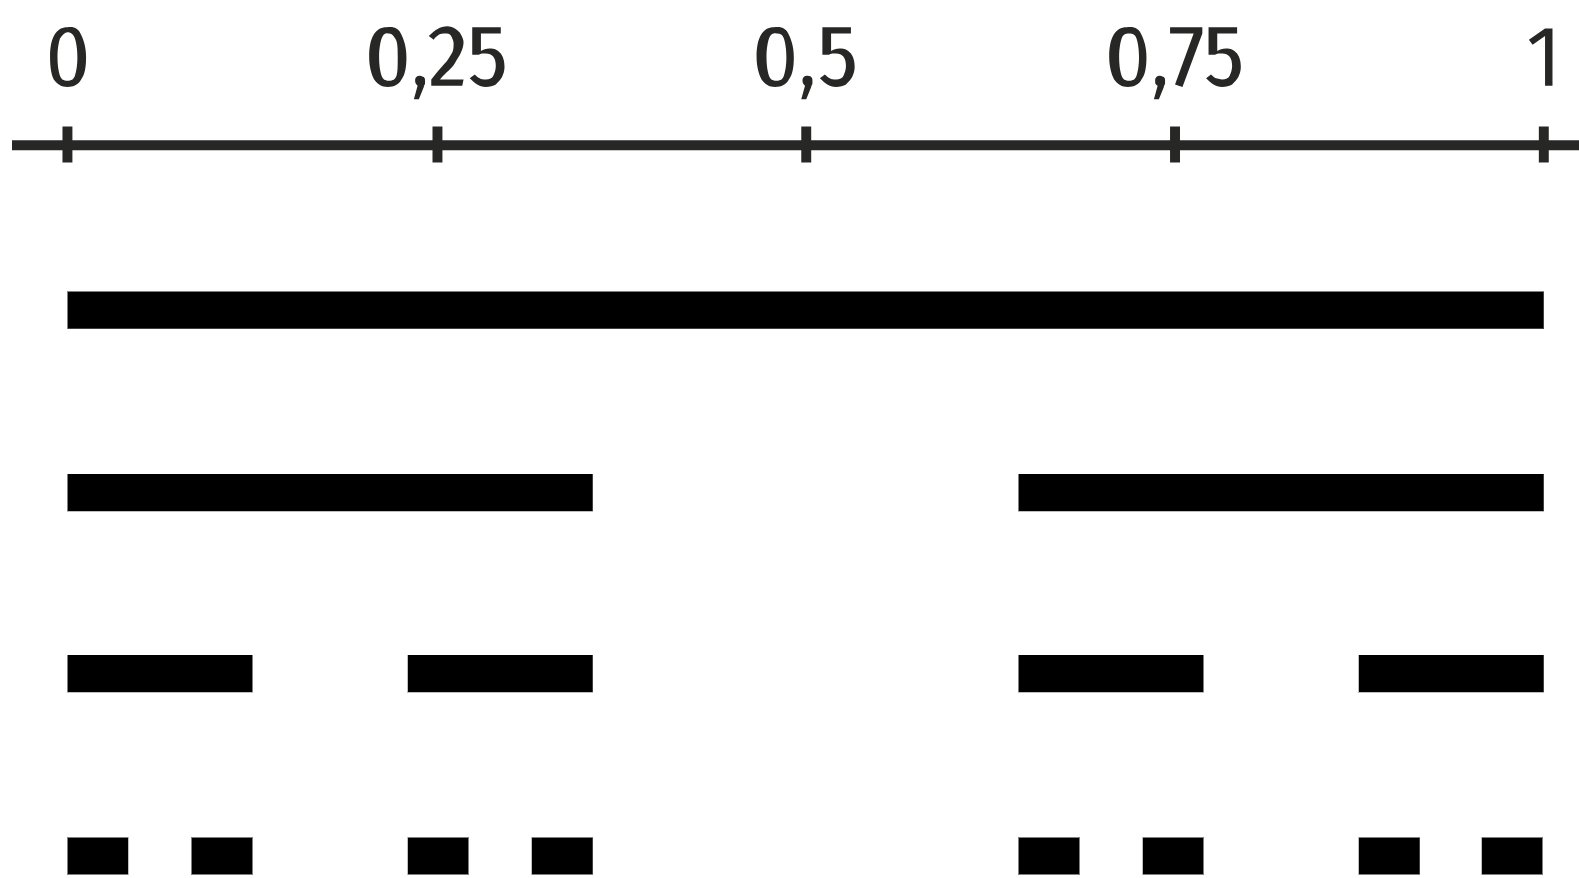
\includegraphics[width=7cm]{cantor1}}

Quelle est la longueur des segments dessinés à la $n^{\text{e}}$ étape ?\\
 Quelle est la longueur totale des segments dessinés après $n$ étapes? après une infinité d'étapes ?\\

	\begin{minipage}{14cm}
        \begin{encadrecolore}{Un peu d'histoire}{UGLiBlue}
		\textbf{Georg Cantor (1845-1918)} était un mathématicien allemand. Il est le fondateur de la théorie des ensembles. Il a démontré en particulier que l'intervalle [0 ; 1] (l'ensemble de tous les nombres réels compris entre 0 et 1) contient plus de nombres que l'ensemble $\N$ et que l'ensemble $\Z$ contient autant de nombres que $\N$.
    \end{encadrecolore}
	\end{minipage}
	\begin{minipage}{3cm}
		\flushright
		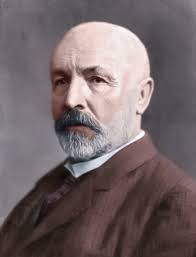
\includegraphics[width=2.5cm]{cantor2}\\
	\end{minipage}

\classe{\premiere spé}
\titre{Nombres hexagonaux}
\maketitle

On construit une suite de figures géométriques en partant d'un point et en ajoutant des points à chaque étape :\\

\includegraphics[width=17cm]{Nb_hexagonaux.jpg}

Combien de points faut-il pour construire la figure à la $n^{\text{e}}$ étape ?\\

\vspace*{3cm}

\titre{Nombres octogonaux}
\maketitle

On construit une suite de figures géométriques en partant d'un point et en ajoutant des points à chaque étape :\\
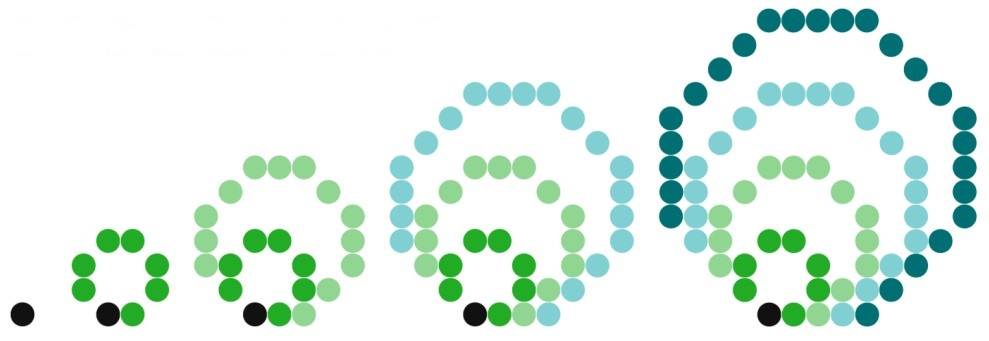
\includegraphics[width=17cm]{Nb_octogonaux.jpg}

Combien de points faut-il pour construire la figure à la $n^{\text{e}}$ étape ?\\

\newpage

\titre{Nombres pentagonaux}
\maketitle

On construit une suite de figures géométriques en partant d'un point et en ajoutant des points à chaque étape :\\
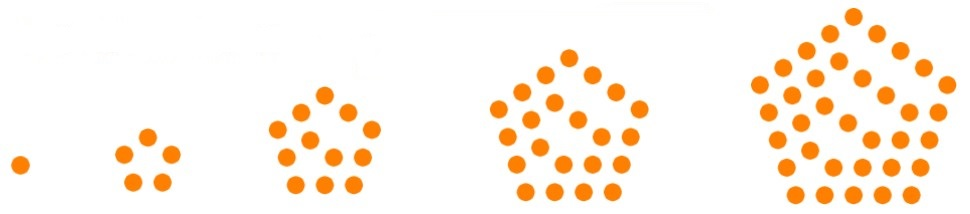
\includegraphics[width=17cm]{Nb_pentagonaux.jpg}

Combien de points faut-il pour construire la figure à la $n^{\text{e}}$ étape ?\\

\vspace*{1cm}

\titre{Coloriage d'un carré}
\maketitle

\dleft{12cm}{
    On colorie un carré en suivant le schéma ci-contre :
    \begin{enumerate}[label=\textbullet]
        \item À l'étape 1, on colorie un quart du carré ;
        \item À l'étape 2, on colorie un quart du quart supérieur ;
        \item Etc.
    \end{enumerate}
    Quelle est l'aire totale des parties coloriées après $n$ étapes ?\\
    Quelle sera l'aire totale des parties coloriées après un nombre infini d'étapes ?}
{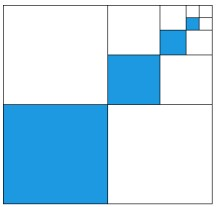
\includegraphics[width=4.5cm]{Carre.jpg}}

\vspace*{1cm}

\titre{Coloriage d'un triangle}
\maketitle

\dleft{12cm}{
    On colorie un triangle en suivant le schéma ci-contre :
    \begin{enumerate}[label=\textbullet]
        \item À l'étape 1, on colorie un quart du triangle ;
        \item À l'étape 2, on colorie un quart du quart supérieur ;
        \item Etc.
    \end{enumerate}
    Quelle est l'aire totale des parties coloriées après $n$ étapes ?\\
    Quelle sera l'aire totale des parties coloriées après un nombre infini d'étapes ?}
{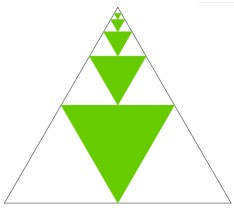
\includegraphics[width=4.5cm]{Triangle.jpg}}

\end{document}

\begin{tikzpicture}[scale = 2.5]
    \draw (0,0) rectangle (2,2);
    % Loop to draw squares of different sizes
    \foreach \i in {0,...,10} {
      \pgfmathsetmacro\side{2^(-\i)}
      \draw[fill=UGLiBlue] (\side,\side) rectangle (2*\side, 2*\side);
      \draw[fill=UGLiGreen] (0,\side) rectangle (\side, 2*\side);
      \draw[fill=UGLiOrange] (\side,0) rectangle (2*\side, \side);
    }
  \end{tikzpicture}
